\chapter{CAP Theorem issue}

In order to optimize performance for the anticipated high volume of read operations, it is essential to prioritize both high availability and low latency in the design of this application. Additionally, it is crucial that the system remains functional in the event of a partition.According to the CAP theorem, the design of this application should prioritize \textbf{Availability (A)} and \textbf{Partition Tolerance (P)} over Consistency (C). This means that the application is more focused on maintaining access to the system and tolerating partitioning rather than ensuring complete consistency of data.
\begin{figure}[H]
	\centering
	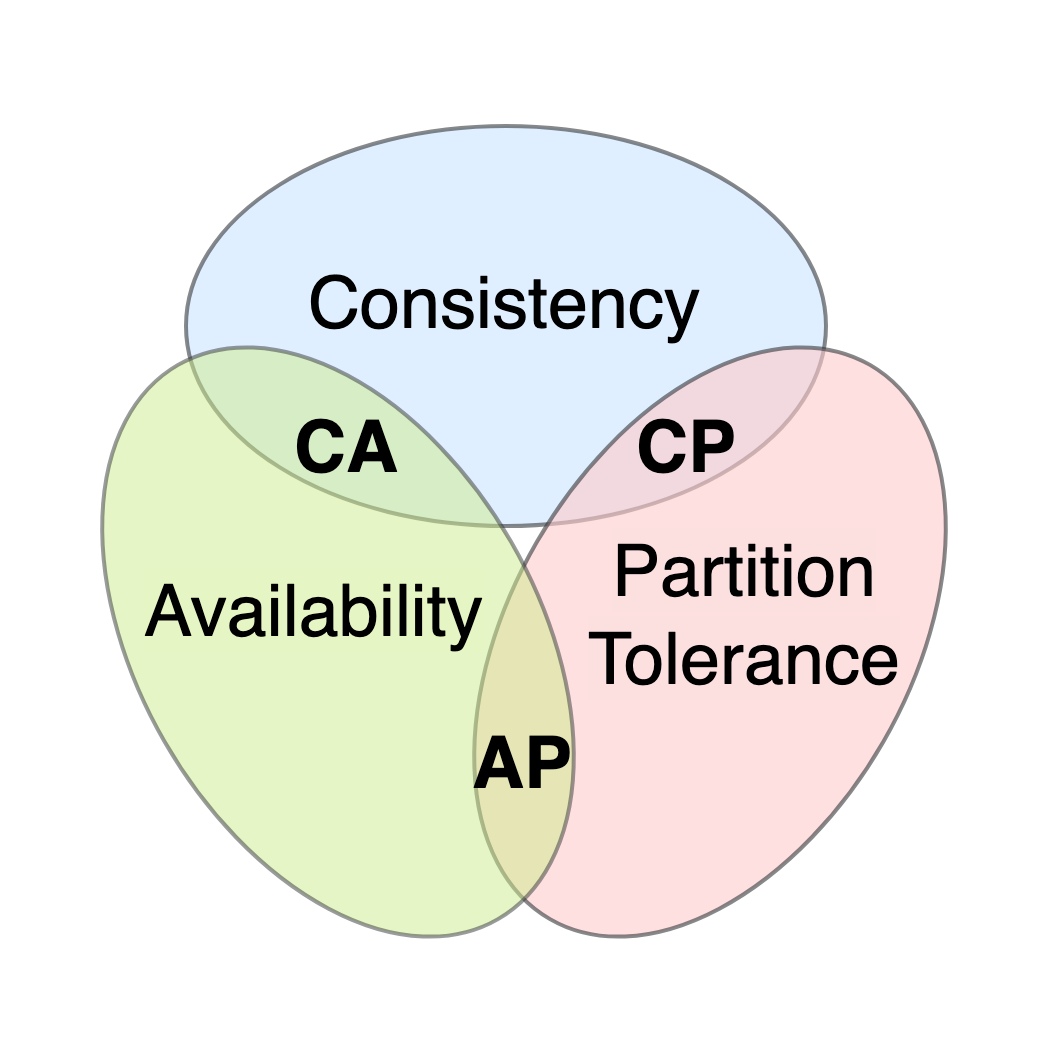
\includegraphics[width=0.4\linewidth]{assets/CAP_Theorem_Venn_Diagram}
	\caption{CAP theorem Venn diagram}
	\label{fig:captheoremvenndiagram}
\end{figure}